\chapter{Datasets}
\label{ch:datasets}

In this section, we first give an overview on the available datasets of annotated news comments. Afterwards, we describe chosen datasets in detail and reflect on the ethics of their creation process.

\section{Datasets of Annotated News Comments}
\label{sec:datasets_comments_table}

In Table~\ref{tab:datasets}, we list the characters of four datasets of annotated news comments. As of the writing, they are the only one available for research purposes.
Since we are not focusing on hate speech detection, we do not include comments datasets about hate speech here.
The interested reader is guided to the datasets section of the survey paper by Schmidt and Wiegand~\cite{schmidt2017survey}.

\begin{table}[H]
\small
  \caption{Four corpora of annotated news comments are available for research.}
  \begin{tabular}{| p{3cm} | p{1.5cm} | p{3cm} | p{5.5cm} |}
    \hline
    Dataset & Language & Unlabeled & Labeled \\ \hline
    SFU Opinion and Comments Corpus (SOCC) &  English & 10k articles, 663k comments from 303k comment threads & 1k comments in responses to 10 articles, labeled for constructiveness and toxicity \\ \hline
    Yahoo News Annotated Comments Corpus (YNACC) &  English & 230k comments from 34k threads under 2.8k articles (not included) & 9.2k comments labeled for agreement, audience, persuasiveness, sentiment, tone, off-topic (15 sub-classes)\\ \hline
        One Million Posts Corpus (OMPC) &  German & 12k articles, 1M comments & 11k comments with the following labels: sentiment, off-topic, inappropriate, discriminating, feedback, personal studies, argument used \\ \hline
        Tencent News Corpus (TNC) &  Chinese &  200K articles and 4.5M comments & 40k comments labeled for quality (from 1 to 5) \\ \hline
  \end{tabular}
  \label{tab:datasets}
\end{table}

Besides the labeled comments, all corpora contain a large number of unlabeled comments. This is helpful for our language-model-based approach. For our experiments, the Yahoo News Annotated Comments Corpus (YNACC) by Napoles et al.~\cite{napoles2017finding} and the One Million Posts Corpus (OMPC) by Schabus et al.~\cite{schabus_academic-industrial_nodate,Schabus:2017:OMP:3077136.3080711} are especially interesting. The number of annotated comments in the SFU Opinion and Comments Corpus (SOCC) by Kolhatkar et al.~\cite{kolhatkar2018sfu} is too small. The Tencent News Corpus by Qin et al.~\cite{2018arXiv180503668Q} has enough data but only one label for quality.
In addition it is in Chinese which makes it harder to work with the text, since we do not read it.
YNACC and OMPC have also some overlapping annotation criteria: off-topic and sentiment. This allows us to compare the same method with identical labels on both datasets.

\section{Yahoo News Annotated Comments Corpus}
\label{sec:datasets_ynacc}

First, we describe characteristics of the data and how it was annotated.
Then, we present reported values and speculate about used metrics. Finally, we explain required data cleaning steps.

\subsection{Description of the Dataset and Annotation Process}
\label{subsec:datasets_ynacc_description}

\begin{wrapfigure}[24]{r}{0.48\textwidth}
  \begin{center}
    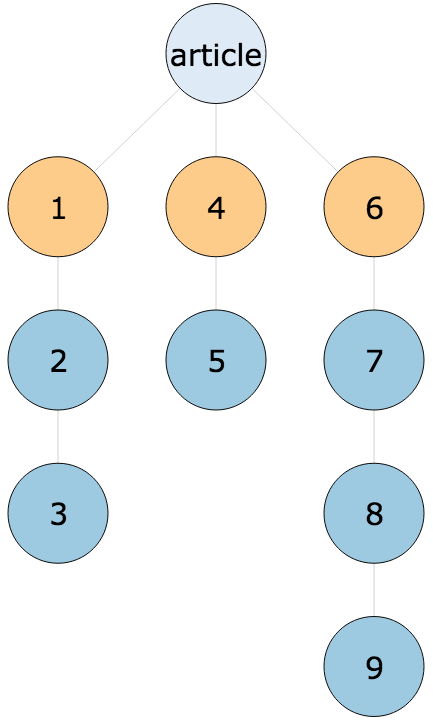
\includegraphics[width=0.36\textwidth]{images/datasets/sequential_structure.png}
  \end{center}
  \caption{The comments 1, 4 and 6 are top-level comments, all others are replies.}
\end{wrapfigure}

The online web service provider Yahoo operates a news outlet called Yahoo News\footnote{\url{https://news.yahoo.com}}. They do not produce own news stories but feature the stories of other outlets. They cover a broad range of topic from politics, to sports to lifestyle. Readers can comment under the articles and there are two types of comments.
There are \textit{top-level comments} that are directly sequential under the article and \textit{replies} that follow-up on a top-level comment.
Unlike other web services such as Reddit, there is no tree-structure. There is only a sequential flow of top-level comments under the article. And each top-level comment can have a sequential flow of replies. The authors used the term \textit{sub-dialogue} to describe a top-level comment including all its replies.

Napoles et al. collected over 230k comments from over 34k sub-dialogues under over 2.8k articles. The comments were written between August 2014 to May 2016. For a subset of 9160 comments, they employed annotators to label them. The dataset contains the comment identifier for training, validation, and test set in a ratio of about $87\%$, $6\%$ and $6\%$. It is worth mentioning that there are different groups of annotators for training and validation, and the test set. The authors used crowd workers to annotate the comments from the training and validation set. Different `Expert annotators' were employed to code the test set.
The comments were annotated on the sub-dialogue level as well as the comment level.
In this master's thesis, we focus on the comment level and therefore neglect the sub-dialogue annotations.
Originally, the authors annotated for over 15 categories but refined to nine categories afterwards. We quote from the annotator notes\footnote{\url{https://github.com/cnap/ynacc/blob/master/rater-guidelines.pdf}} to describe the different classes:
\begin{description}
    \item \item [Persuasive] ``This is an opinion based on whether you think the user means to be persuasive and how persuasive they seem to be. Generally, the commenter incorporates new information or a personal story, or uses specific language in attempt to convince other users of his or her point. In order for a comment to have true persuasiveness, they must present a well-reasoned argument.''
    \item [Audience] ``Choose whether the comment is meant to be 1) a reply to a specific commenter; 2) broadcast message/general audience; [..] Please note that a top-level comment with ALWAYS be a broadcast message with a general audience, by nature of being a top-level comment.''
	\item [Agreement] ``Agreement with other commenter: The comment indicates agreement with either another commenter explicitly, meaning, the user is clearly expressing they agree with another person or point of view in the thread. Can occur concurrently with other types of agreement/ disagreement.''
	\item [Informative] ``Informative (Constructive, Productive): This comment furthers the discussion by adding new information. Usually an attempt to be persuasive and convince others of the user's argument. It may be passionate, but it is not dismissive. NOT a personal story. Criteria for informativeness: 1. Mention of historical facts or evidence 2. Mention of statistics and other numbers 3. Quote or paraphrase of public discourse made by a popular figure 4. Mention of events, or `news' 5. Presenting a cogent or logical analysis or argument''
	\item [Mean] ``Mean (Hateful): The comment is intended to be rude, mean, or hateful with no other intent. Be careful to not assign this to comments you personally disagree with. Note that mean, hateful comments/insults can still be on topic with the article or conversation.''
	\item [Controversial] ``Controversial (Outspoken): This comment puts forth a strong opinion in a way that others will certainly strongly disagree with.''
	\item [Disagreement] ``Disagreement with other commenter: The comment indicates disagreement with either [sic] another commenter. Can occur concurrently with other types of agreement/ disagreement.''
	\item [Off-topic] ``Off topic with article: The conversation/contributions have begun to be irrelevant to the article (Also can be thought of as a digression). Each contribution that is off topic to the article once an off-topic conversation has begun should get an `off-topic' flag. Once a digression begins, every contribution within the digression is on topic with that conversation but OFF topic with the article.''
	\item [Sentiment]
		Positive: ``A positive sentiment generally expresses feelings of positive emotion, for example `I love the Yankees! Gunna be a great year.' When users express their opinion on something as being great or good, this is a positive sentiment. Attempts at making jokes or at being funny to `lift the mood' generally have a positive sentiment, unless they are mean-spirited.''
		
		Negative: ``A negative sentiment is more common and indicates the commenter is unhappy for some reason. Usually goes in hand with some complaint about the world or the issue. For example, `Donald Trump sucks. I can't believe he's allowed to be in the public eye.' Additionally, mean or controversial comments are usually coming from a negative emotional place on the part of the commenter. Sarcasm, although funny, is usually used to express discontent or absurdity, is usually negative.''
		
		Neutral: ``A neutral sentiment has no emotion. Usually when a commenter is just stating fact, like `I think the season starts in July, actually.' or `If you water your basil every day, it shouldn't die'.''
		
		Mixed: ``A mixed sentiment is when a user seems to express both positive and negative emotion about something or several things. A good example is when a commenter expresses that they are in agreement with something one commenter said, but also is offended or takes issue by something else. Longer comments that contain many expressions of different emotions are usually `mixed'.''
\end{description}


\begin{figure}[h]
    \centering
    \subfloat[Binary Categories]{{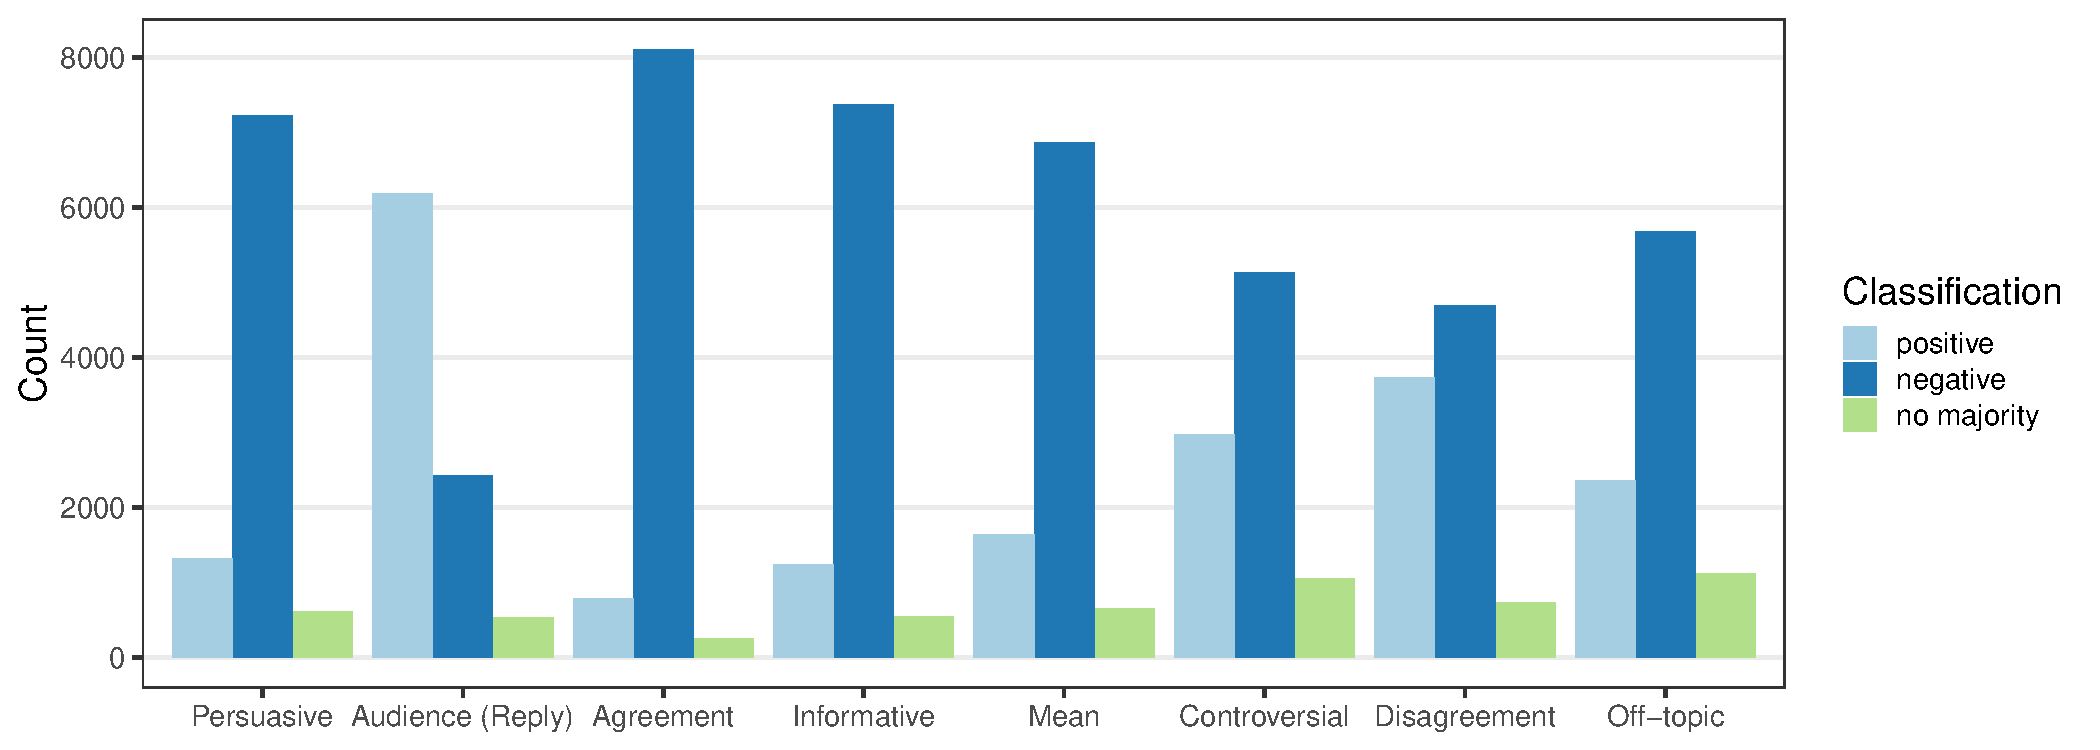
\includegraphics[height=110pt]{graphs/class_distributions/class_dist_ynacc_bin_no_maj} }}
    \subfloat[Sentiment]{{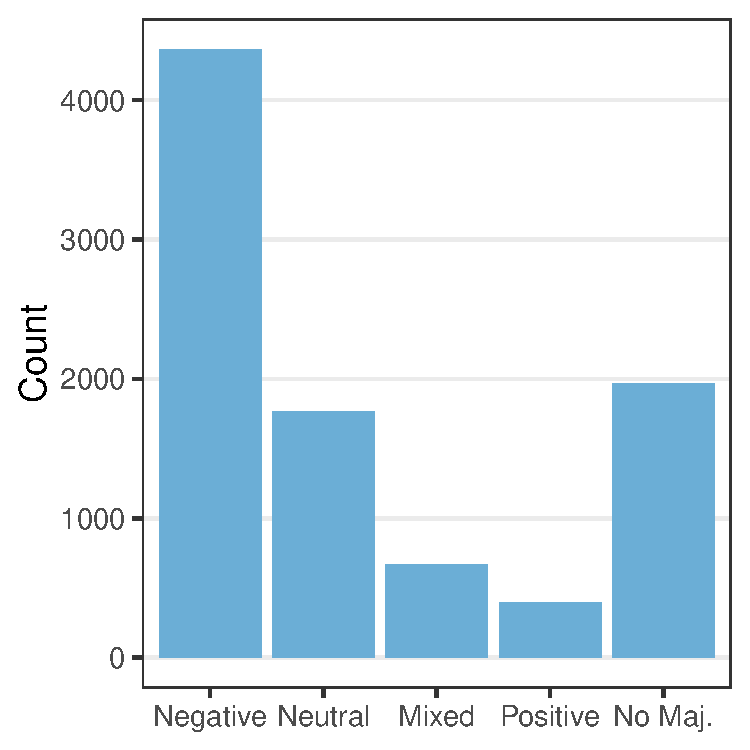
\includegraphics[height=110pt]{graphs/class_distributions/class_dist_ynacc_sentiment_no_maj} }}
    \caption{The distributions for each category where the number of samples without majority vote is present.}
    \label{fig:class_distru_no_maj}
\end{figure}
\begin{figure}[h]
    \centering
    \subfloat[binary categories]{{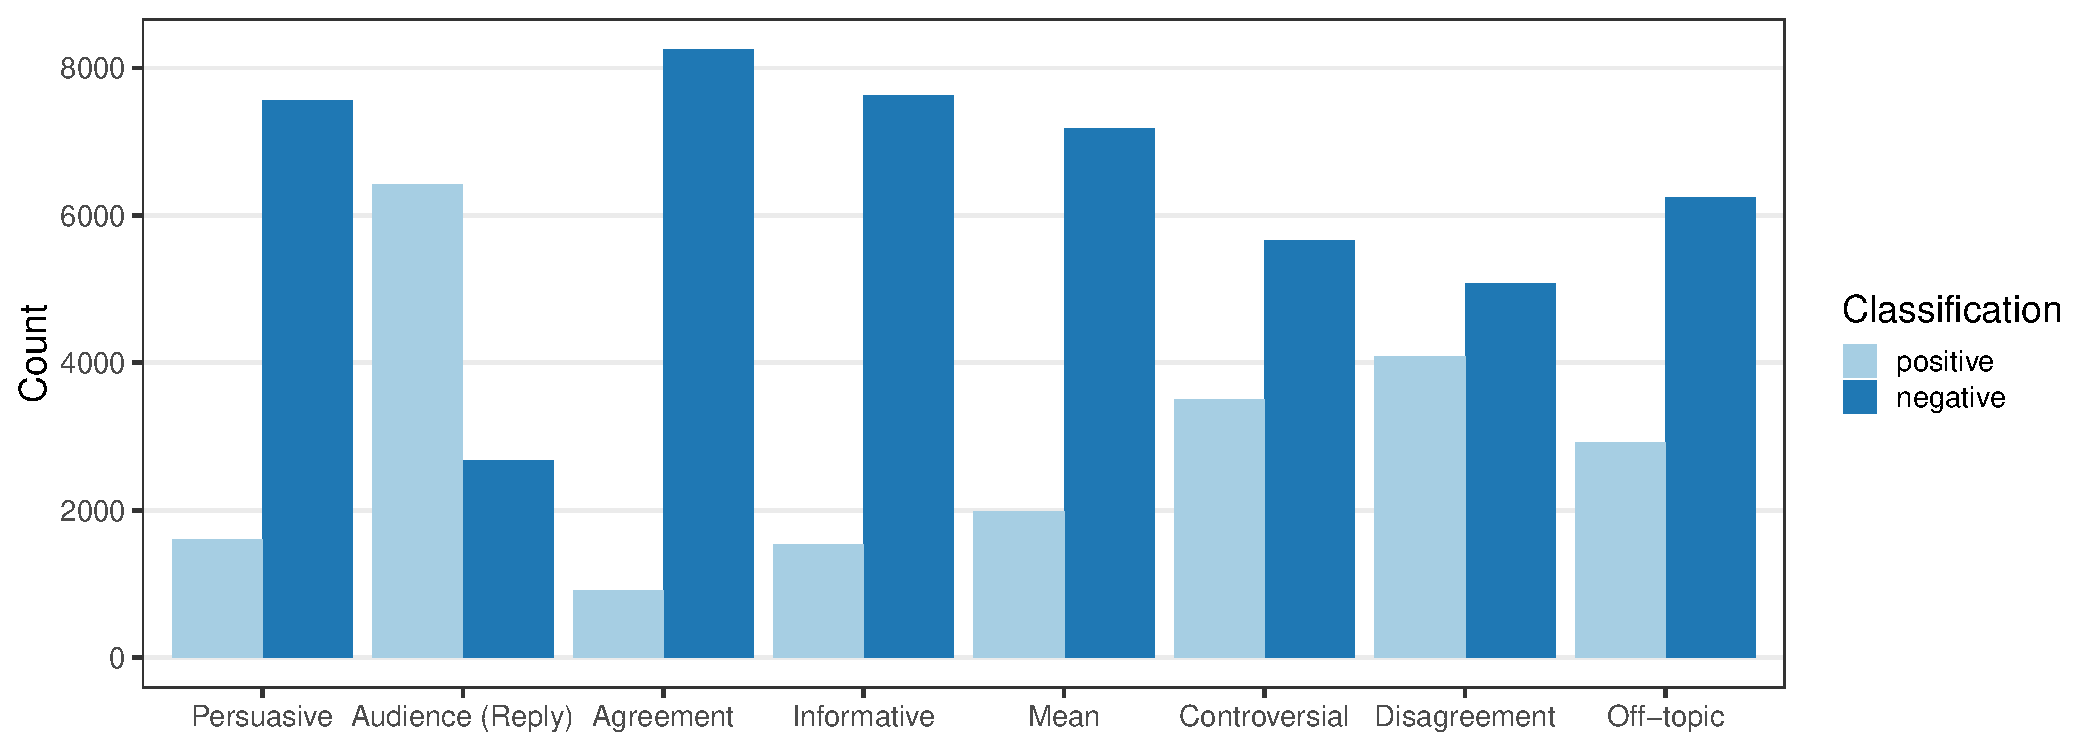
\includegraphics[height=110pt]{graphs/class_distributions/class_dist_ynacc_bin} }}
    \subfloat[Sentiment]{{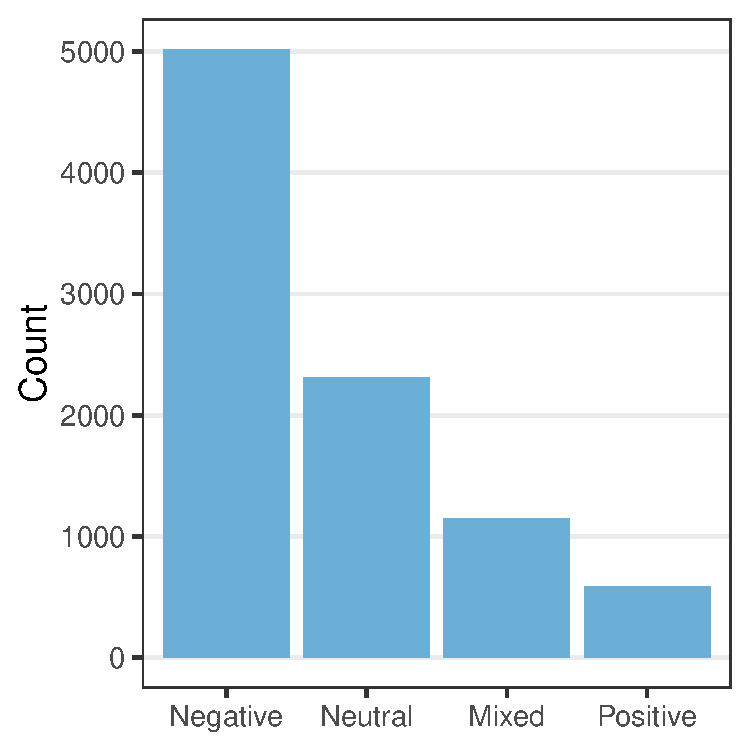
\includegraphics[height=110pt]{graphs/class_distributions/class_dist_ynacc_sentiment} }}
    \caption{The final distributions for each category.}
    \label{fig:class_distru}
\end{figure}

Napoles et al. only publish the raw annotations\footnote{\url{https://webscope.sandbox.yahoo.com/catalog.php?datatype=l&did=83}} for each annotator.
So for using the data for classification, one has to consolidate the annotations to derive a final assessment.
In the authors' follow-up work~\cite{napoles2017automatically}, they choose a majority vote for each sample. If there is no majority for a class, they randomly choose an applicable class, according to the authors' post on GitHub\footnote{\url{https://github.com/cnap/ynacc/issues/2}}. Consequently, to compare results, it is advised to replicate their approach.
In Figure~\ref{fig:class_distru_no_maj} is the number is the number of undecided samples visualized.
The binary categories Controversial and Off-topic have the largest share of un-decided samples.
Over 1000 samples, almost 10\% of the data, are randomly assigned to classes.
While the share for Sentiment is large as well, it is a four-class setup so dissension is more likely.
The random selection is done for each applicable label.
So undecided samples do not get uniformly distributed over the four classes.
In Figure~\ref{fig:class_distru} is the final outcome of this procedure shown.
As it is often the case with real-life data, the distributions are mostly imbalanced.
Agreement is the most imbalanced while Disagreement is almost balanced.

\begin{figure}
    \centering
    \subfloat[unlabeled comments (YC\textsubscript{LM})]{{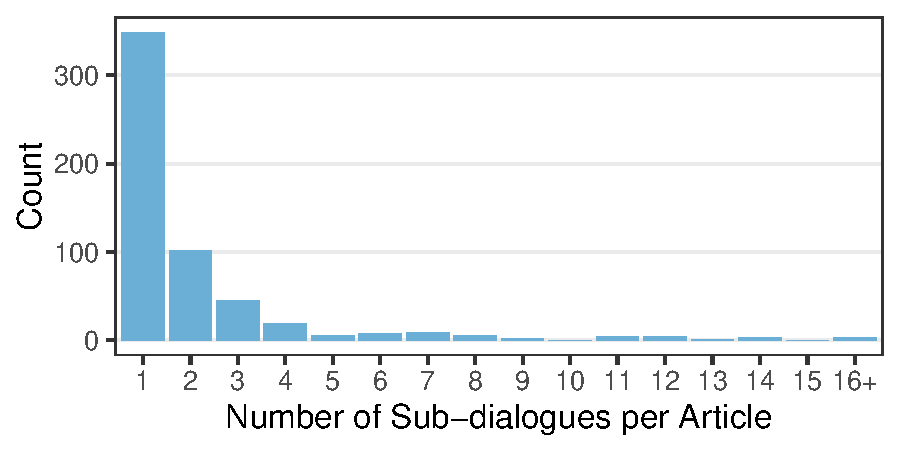
\includegraphics[width=0.5\textwidth]{graphs/eda/threads_per_article_cl} }}
    \subfloat[annotated comments (YC\textsubscript{CL})]{{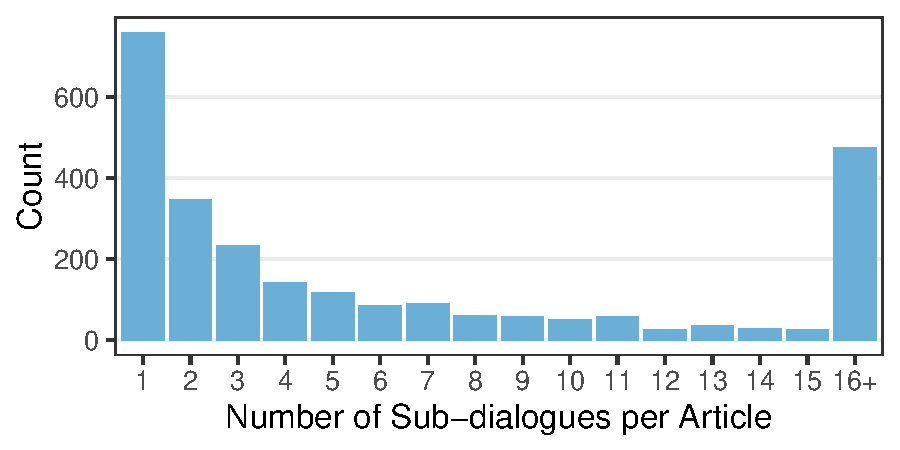
\includegraphics[width=0.5\textwidth]{graphs/eda/threads_per_article_lm} }}
    \caption{The number of sub-dialogues per article.}
    \label{fig:threads_per_article}
\end{figure}

In addition to the annotated comments, the YNACC contains a large number of unlabeled comments.
After cleaning the data, as it will be described in Subsection~\ref{subsec:ynacc_data_cleaning}, about 238k unique comments remain.
As we will train a language model which does not require annotations, the unlabeled is also part of this work.
In the following, we provide several graphs comparing the characteristics of unlabeled comment set, we denote as YC\textsubscript{LM} with the portion of labelled training data YC\textsubscript{CL}.
In Figure~\ref{fig:threads_per_article} is the number of sub-dialogues per article are shown.
There is a stark difference between the two sets of comments with a lot more articles having only one annotated sub-dialogue. In Figure~\ref{fig:replies_per_thread} is the the frequency of number of replies for each top-level comments.
There are only a fews comments in the columns 0--2.
This is most likely the reason for some sampling. In Figure~\ref{fig:threads_per_article} the frequency of comments per rank is displayed. Here ranks refers to the distance to the parent comment. The top-level comments have a rank of 0 and no parent comments. While the information is the same in both graphs, Figure~\ref{fig:threads_per_article} gives a better feeling of how large the share of comments on the early ranks is. Finally, to get a better sense of YC\textsubscript{LM}, we list the 30 most frequent tokens in Figure~\ref{fig:word_freq}, excluding stop words and tokens with a length of three or less.
In Figure~\ref{fig:len_com} is the number of tokens for the comments. This allows to truncate the comments to abolish outliers. And since word based approaches rely on fixed vocabulary, we plot the share of all token covered by choosing only N most frequent tokens in Figure~\ref{fig:vocab_size}.

\begin{figure}
    \centering
    \subfloat[Unlabeled comments (YC\textsubscript{LM}).]{{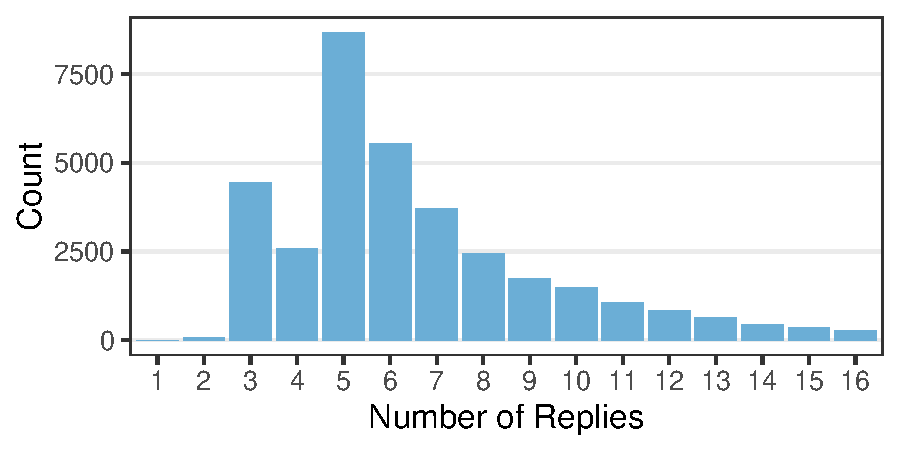
\includegraphics[width=0.5\textwidth]{graphs/eda/lm_num_replies} }}
    \subfloat[Annotated comments (YC\textsubscript{CL}).]{{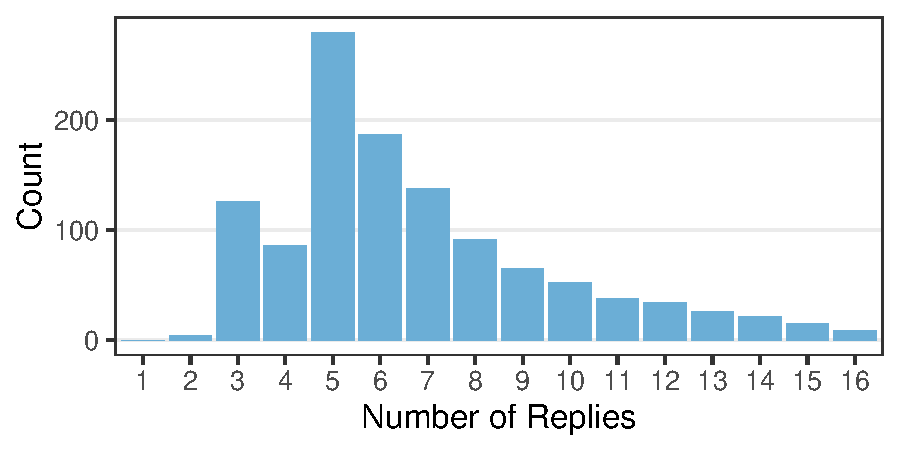
\includegraphics[width=0.5\textwidth]{graphs/eda/cl_num_replies} }}
    \caption{Frequency of number of replies for each top-level comment.}
    \label{fig:replies_per_thread}
\end{figure}

\begin{figure}
    \centering
    \subfloat[Unlabeled comments (YC\textsubscript{LM}).]{{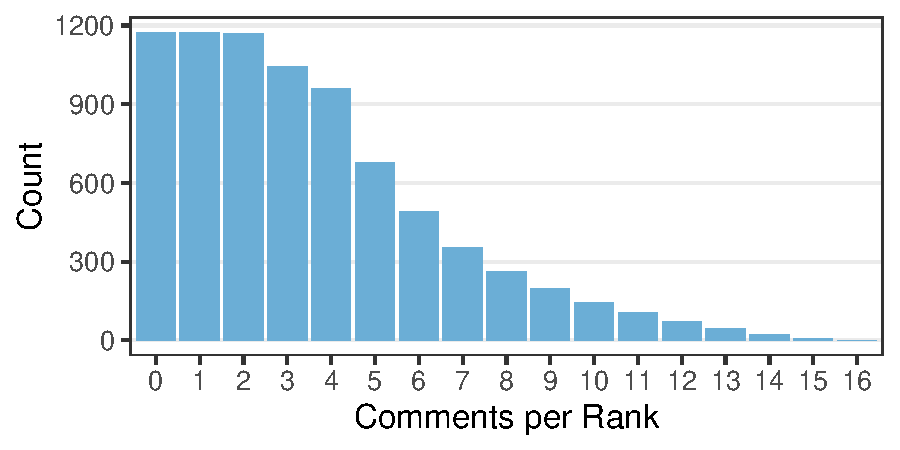
\includegraphics[width=0.5\textwidth]{graphs/eda/comments_per_rank_cl} }}
    \subfloat[Annotated comments (YC\textsubscript{CL}).]{{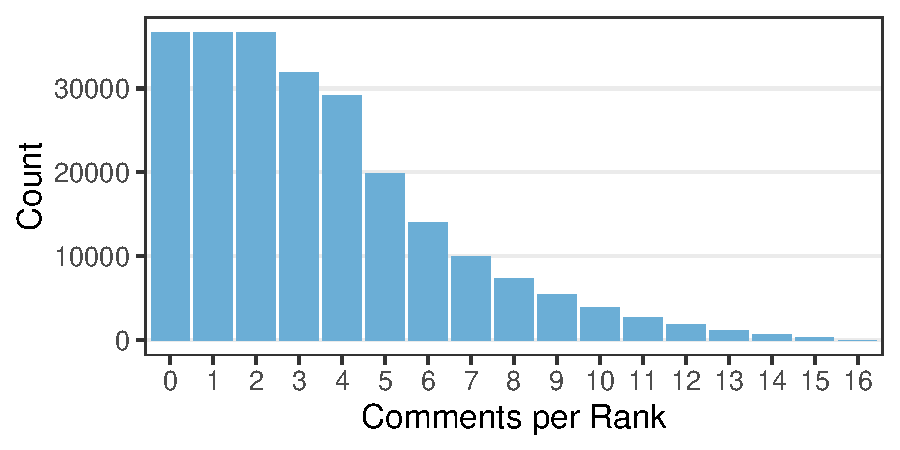
\includegraphics[width=0.5\textwidth]{graphs/eda/comments_per_rank_lm} }}
    \caption{Frequency of comments per rank.}
    \label{fig:comments_per_rank}
\end{figure}

\begin{figure}
    \centering
    \subfloat[Number of tokens in a comment, truncated at 300.\label{fig:len_com}]{{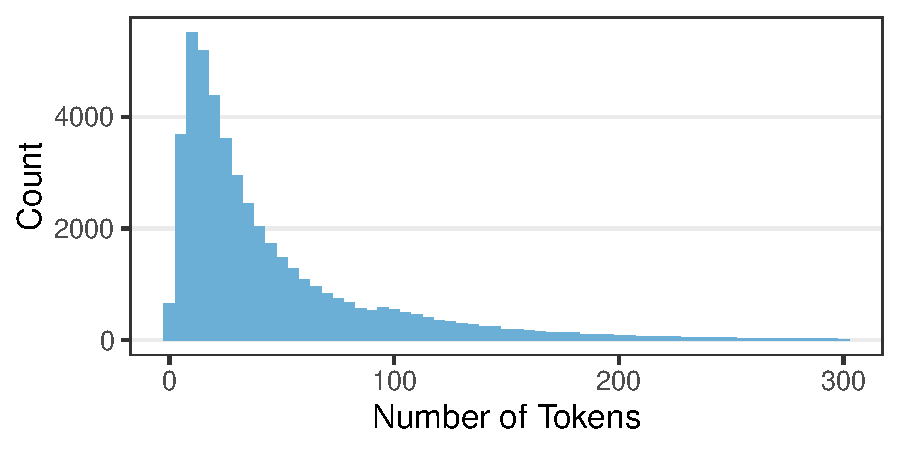
\includegraphics[width=0.5\textwidth]{graphs/eda/comment_length} }}
    \subfloat[Share of text covered by fixed vocabulary size.\label{fig:vocab_size}]{{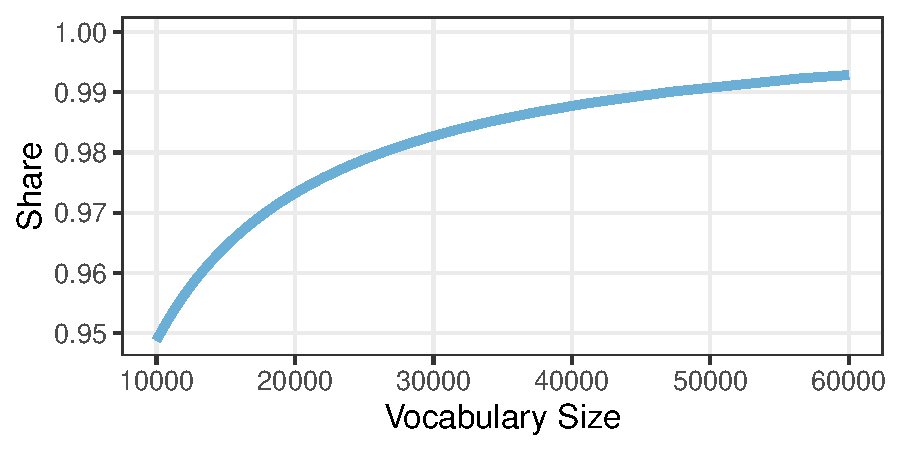
\includegraphics[width=0.5\textwidth]{graphs/eda/max_vocab} }}
    \caption{Text analysis of YC\textsubscript{LM}.}
    \label{fig:word_based_anal}
\end{figure}

Besides the text, each comment has the number of up-votes, timestamp, parent comment id (if it is a reply), and the article's headline and URL. The article text is not part of the datasets. We were able to crawl about 80 percent of the article  texts to not limit ourselves to the headline. Since a lot of articles are offline, we resorted to the Internet Archive's Wayback Machine\footnote{\url{https://archive.org/web/}} to fetch them.
The data of the articles were extracted using the Python package Newspaper3k\footnote{\url{https://github.com/codelucas/newspaper}}.
Information about the comment's author is also not part of the datasets.
In addition, all mentions of usernames were replaced by the token \textit{@username}.

%\vspace{-25pt} %no idea if useful
\begin{wrapfigure}[16]{r}[-5pt]{0.4\textwidth}
  \begin{center}
    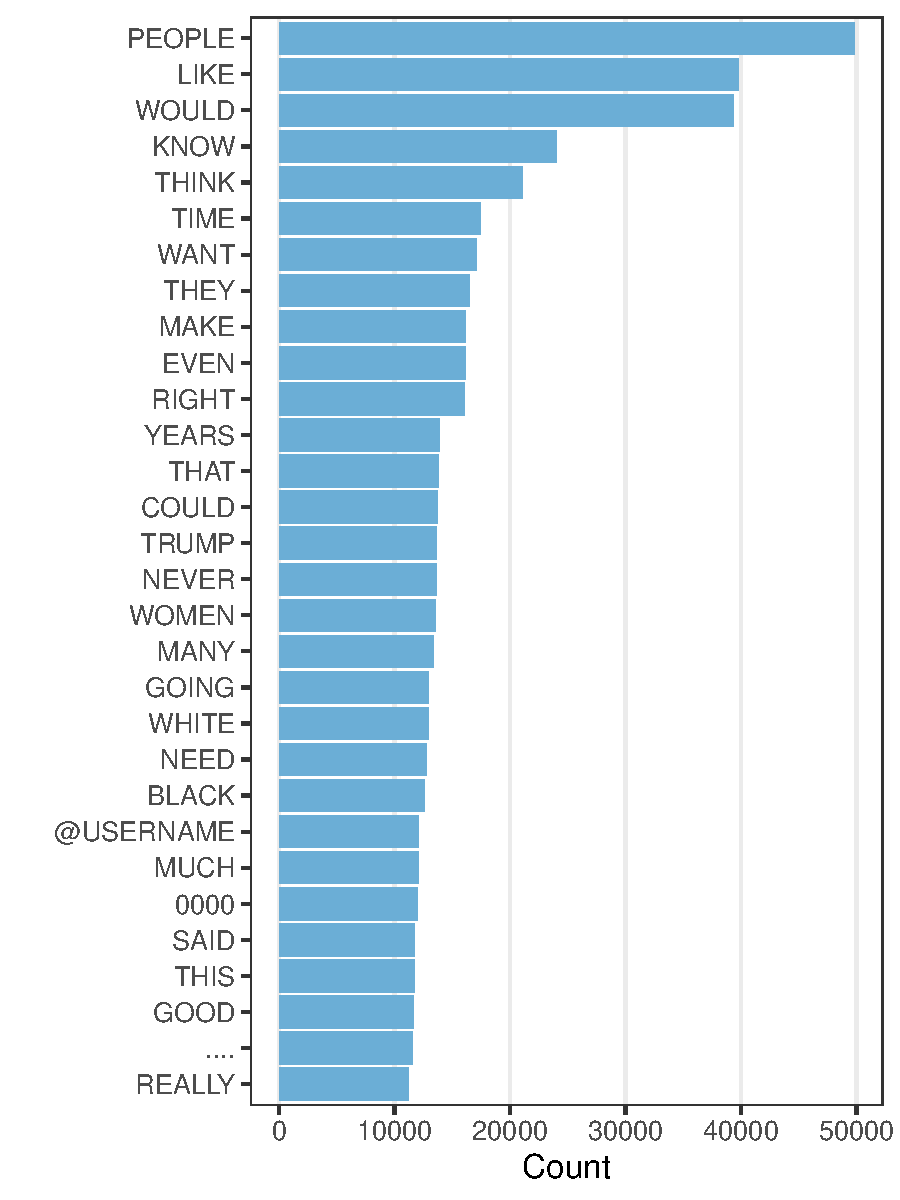
\includegraphics[width=0.36\textwidth]{graphs/eda/word_freq}
  \end{center}
  \caption{The 30 most frequent tokens in YNACC.}
  \label{fig:word_freq}
\end{wrapfigure}

\subsection{Data Cleaning}
\label{subsec:ynacc_data_cleaning}

The provided data is `dirty'.
There are duplicated rows as well as corrupted text encodings.
In addition, due to the nature of user-generated text, there are other issues, e.g., different forms of quotation marks. So first, the text is cleaned with the Python package \textit{clean-text}\footnote{\url{https://github.com/jfilter/clean-text}. The package was developed over the course of this master's thesis and borrows code from another Python package textacy: \url{https://github.com/chartbeat-labs/textacy}.} in the following way: whitespaces are normalized but (single) newlines are kept, UTF8 encoding issues are fixed, the text is transliterated to ASCII and the casing is kept. All digits are replaced by a `0'.
Then, duplicated rows were removed.
First, duplicates based on comment ID and text were deleted.
Second, rows with duplicated ID but different text were cleaned.
This situation occurred because some characters such as quotations marks were stripped from some rows.
So in the case of duplicated IDs but different text, we chose the sample with the longest text.

\subsection{Reported Values}
\label{subsec:ynacc_reported}

Napoles et al.~\cite{napoles2017automatically} report in the accompanying publication results for the classification of individual comments.
Even though the focus are predictions on thread-level.
Unfortunately, it is unclear which kind of metrics they used and they also did not respond to our email.
They only write that they use precision, recall and $\text{F}_{1}$ score.
We report their values in Table~\ref{tab:ynacc_reported} and try to convert their values into our metric of choice: Cohen's Kappa.
We gave background information about metrics for classification and shortcomings of the $\text{F}_{1}$ score in Section~\ref{sec:metrics}.

\begin{table}
\nprounddigits{3}
\small
\centering
\caption{Reported Results on YNACC and their conversation into Cohen's Kappa.}
\label{tab:ynacc_reported}
\begin{tabular}{l l l l  n{1}{3} n{1}{3} n{1}{3} n{1}{3} n{1}{3} n{1}{3}}
\toprule
\multicolumn{1}{l}{} & \multicolumn{3}{c}{Reported} & \multicolumn{6}{c}{Calculated} \\
\cmidrule(r){2-4}
\cmidrule(r){5-10}
\multicolumn{4}{l}{} & \multicolumn{3}{c}{Presence = Positive} & \multicolumn{3}{c}{Absence = Positive} \\
%\cmidrule(r){2-4}
\cmidrule(r){5-7}
\cmidrule(r){8-10}
\multicolumn{1}{l}{Category} & \multicolumn{1}{l}{Precision} & \multicolumn{1}{l}{Recall} & \multicolumn{1}{l}{F\textsubscript{1 binary}} & \multicolumn{1}{l}{F\textsubscript{1 micro}} & {F\textsubscript{1 macro}} & {Kappa} & \multicolumn{1}{l}{F\textsubscript{1 micro}} & {F\textsubscript{1 macro}} & {Kappa}  \\
\midrule
Persuasive & $0.81$ & $0.84$ & $0.91$ & 0.9468267581475128 & 0.8947953594234788 & 0.7896017415802279 & 0.7013422818791947 & 0.41222879684418146 & -0.17343597911689246 \\
Audience & $0.80$ & $0.99$ & $0.88$ & 0.8296041308089501 & 0.7808674781416081 & 0.5751386806319849 & 0.9122203098106713 & 0.9071317756569979 & 0.8155406288713061 \\
Agreement & $0.69$ & $0.85$ & $0.76$ & 0.9382504288164666 & 0.8638274680784803 & 0.7281065395377759 & 0.6151685393258427 & 0.38086956521739135 & -0.1841456752655537 \\
Informative  & $0.76$ & $0.74$ & $0.75$ & 0.9193825042881647 & 0.8516081515057974 & 0.7032307675645233 & 0.5990016638935108 & 0.3746097814776275 & -0.249868404021228 \\
Mean & $0.74$ & $0.78$ & $0.75$ & 0.8970840480274442 & 0.6798847989117535 & 0.6927536231884058 & 0.6112054329371817 & 0.37934668071654365 & -0.23774696484450275 \\
Controversial & $0.67$ & $0.64$ & $0.65$ & 0.5746140651801029 & 0.5630107838870352 & 0.15794623305222943 & 0.5420240137221269 & 0.487601591894374 & -0.023822834930511405 \\
Disagreement & $0.60$ & $0.68$ & $0.64$ & 0.6878216123499142 & 0.6816769068305093 & 0.36530363210030137 & 0.5385934819897084 & 0.5010102167113708 & 0.008985838773072685 \\
Off-topic & $0.62$ & $0.67$ & $0.61$ & 0.4922813036020583 & 0.3790016121602948 & -0.23743689765947673 & 0.7684391080617495 & 0.7368473845227945 & 0.47409040793825796 \\
%\midrule
Sentiment & 0.44 & 0.46 & 0.43 \\
\bottomrule
\end{tabular}
\end{table}

It seems like the authors did not average the metrics but only chose one class as the positive one. There are several indications for this. Micro-averaged values are ruled out because precision, recall and $\text{F}_{1}$ would be identical.
For macro-averaging, the values would be extremely strong, i.e., with a recall of 0.99 for the category Audience. They could have used weighted average but this is rather uncommon so they would have mentioned it in the paper. So it is more probable that the authors refrained from averaging.
To distinguish this from averaged score, we refer to it as F\textsubscript{1 binary}  in Table~\ref{tab:ynacc_reported}.
The strong performance of recall for Audience may be due to choose the majority class the positives class\footnote{The F\textsubscript{1} differs depending on what class is the positive and what is the negative class.}.
This shows that $\text{F}_{1}$ scores do not always yield meaningful evaluation. As a consequence, we convert the results into Cohen's Kappa. To do so, we reconstruct $fp$, $tp$, $tn$, and $fn$\footnote{These are the acronyms for false positives, true positives, true negatives, false negatives respectively.}. But since the binary metrics are always in respect to one class, that we do not know, we have calculate them for both situations.
So the table consists of values if the original results came from the presence and the absence of a specific class.
We can to the conversation because we have four unknowns and four equations. We have precision and recall.
And since we know the distributions of the classes (because we have the samples), we can derive two additional equations:

\begin{align*}
    class_0 &= tp+fn & class_1 &= fp+tn\\
\end{align*}

This enables us to solve for the four unknown variables. With them, we can calculate a different metric, in this case Kohen's Kappa. But we only do this for the eight binary classes.
The category Sentiment has four classes and thus we cannot reconstruct the original values.
In the original paper, the authors reveal that the results for the categories Informative and Controversial are below a simple ridge regression baseline.

We will continue to discuss the values in the evaluation Section~\ref{sec:exp_ynacc_results} to set our contribution into perspective.

\subsection{Discussion}

There are several issues with the YNACC dataset:
\begin{itemize}
	\item It is unclear what metric was used for the reported values. Since the authors did not reply to our email, we and others researchers can only speculate. This makes it hard to compare results and sets new inventions into perspective.
    \item For the consolidation of annotations, the authors decided to randomly assign samples to classes when there is no majority among the annotators. This adds unnecessary noise. It is most likely better to fully remove the samples from dataset.
    \item The authors did not provide the consolidated assignment for the samples. Therefore, it is not fully clear, how they derived the values. For instance, there are classes marked as `NA'. It is unclear whether they were removed or kept.
    \item Two different groups of people annotated the data. One group annotated training and validation and the other group, ``expert annotators'' the test set. It is true, that the test set is used to evaluate the performance of a model in the wild. However, then the test set cannot be used to asses the performance of the model. A model can only learn what is has been taught.
\end{itemize}

Nevertheless, it is still the largest corpus of publicly available news comments. We follow the setup of the original paper, including the random assignments to compare our results.

\section{One Million Posts Corpus}
\label{sec:ompc_ds}

The One Million Posts Corpus\footnote{\url{https://ofai.github.io/million-post-corpus/}} (OMPC) is a dataset consisting of German comments from the Austrian newspaper \textit{DerStandard}\footnote{\url{https://derstandard.at/}}.
The dataset was presented in-depth in the publication by its creators Schabus et al.~\cite{Schabus:2017:OMP:3077136.3080711} and thus we only give a brief overview.

\begin{figure}
  \begin{center}
    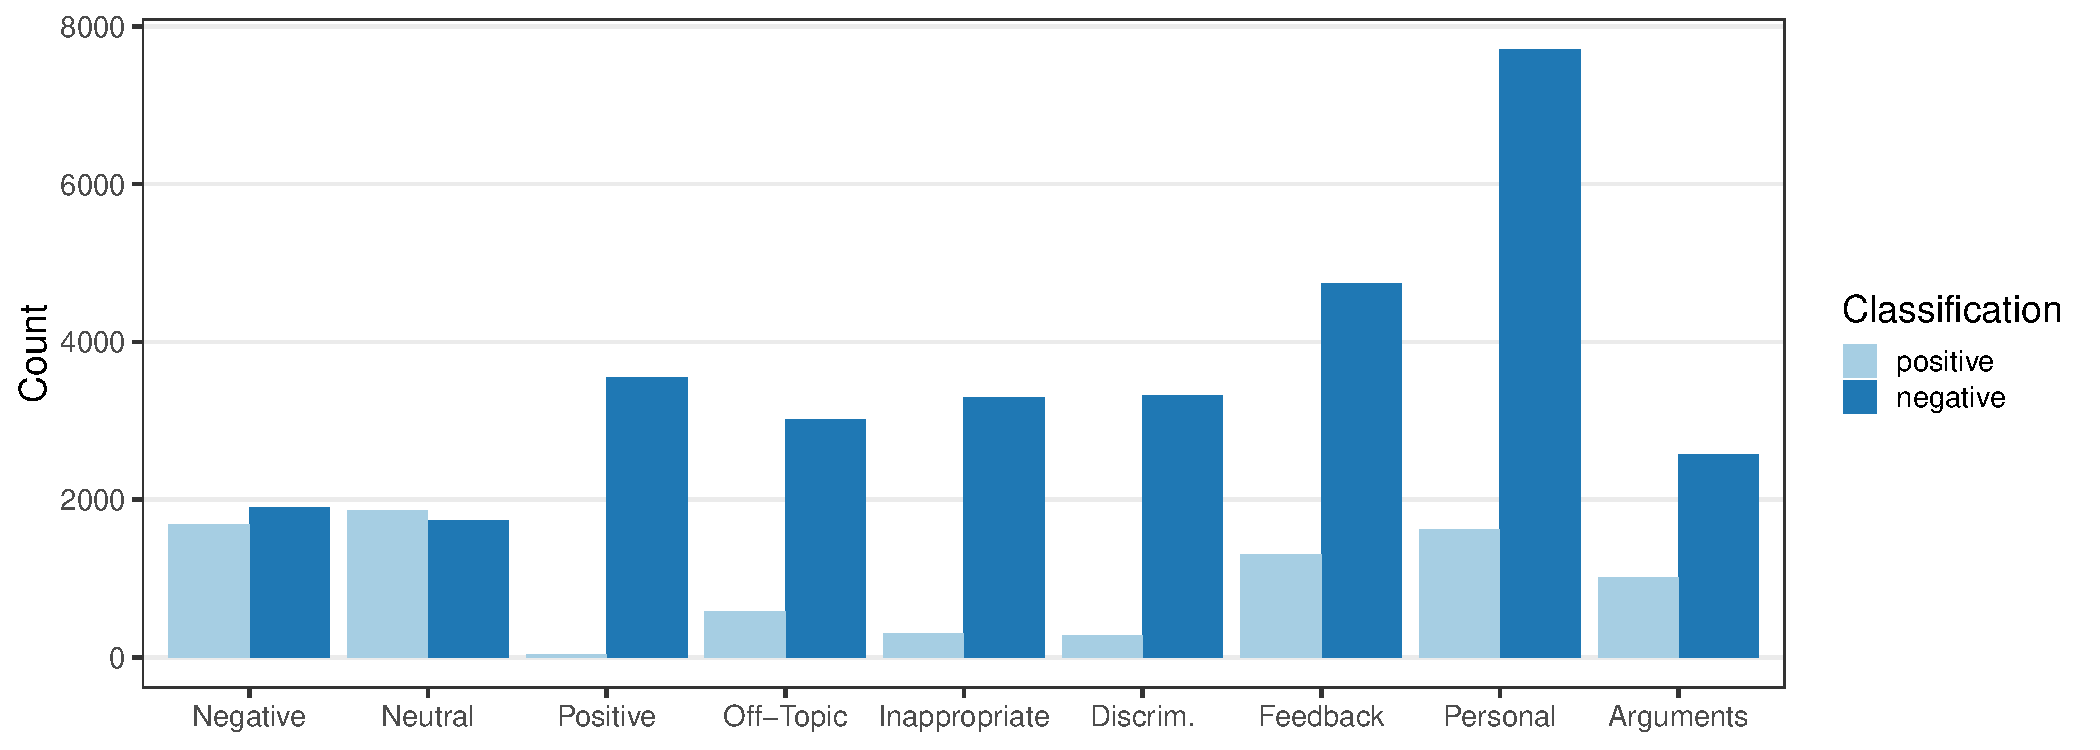
\includegraphics[width=\textwidth]{graphs/class_distributions/class_dist_ompc_bin}
  \end{center}
	\caption{The distributions of classes in OMPC are imbalanced. Also the number of samples varies among the categories.}
   \label{fig:data_ompc_distu}
\end{figure}

It contains 1 million unlabeled comments and 11,773 labeled ones from 2015 to 2016. A comment consists of its text, user votings and pseudonymized author ID but also information about the article is included: the article's text, headline, topic, and timestamps. The comments were labeled by professional comment moderators in seven categories.
One category, sentiment, is annotated into three classes. All others are binary classifications. They are presented as follows:
\begin{description}
	\item[Sentiment] The sentiment of a comment for three classes: positive, neutral or negative. For further use, the category is split up into three binary classification setups and denoted as \textit{positive}, \textit{neutral} and \textit{negative}.
	\item[Off-topic] If a comment is out of the article's topic.
	\item[Inappropriate] If inappropriate words were used, i.e., swearwords.
	\item[Discriminating] If a comment is discriminating, i.e., racist.
	\item[Personal] If it includes a personal story.
	\item[Feedback] If feedback is given to the article's author.
	\item[Arguments] If arguments are used in a comment.
\end{description}

The number of samples per class varies as shown in Figure~\ref{fig:data_ompc_distu}. The sampling process was done in an interactive way, driven by annotating moderators.
Moderators chose articles under which certain kind of comments appeared often.
For instance, under articles about refugees are a lot of racists comments. So they chose comments from these articles for the category Discriminating. This resulted in a strong bias in the data and thus the annotated data were not sampled representatively. As a consequence, not all comments were assigned with the same class (as the different number for each category indicates). In the publication, the authors provide feature-based as well as neural models results as baselines. They will be presented in Section~\ref{sec:ompc_results} to compare them with our experiment results.

\section{Ethical Considerations}

In this section, the creation of the news comments datasets is reflected critically.

A major problem is the fact, that commentators did not consent for being part of the dataset. Their comments get taken out of the context of the newspaper website in which they originally created them. Then it gets added into the dataset that explicitly invites other people to use it (for research or other purposes). The commentators who contributed to the dataset are most probable not even aware of it. ``Recognize that privacy is more than a binary value'' is one of the ``Ten simple rules for responsible big data research'' that a consortium of 13 researches and philosophers~\cite{DBLP:journals/ploscb/ZookBb0KGGH0MNN17} postulated.
Even though the comment is publicly visible on the newspaper's website, does not give computer scientist do not the right to do everything they desire.
In a research context, when working with user-generated content the same research ethics should apply that exists for social scientists or in the medical domain. One guiding principle is that research participants should consent to being part of experiments. This principle is the result of the discussion after crimes against humanity were done in the name of research during the German National Socialism\footnote{The Nuremberg~Code lists ten rules for human experiments in the aftermath of the Nuremberg trials in 1947. \url{https://en.wikipedia.org/wiki/Nuremberg_Code}}. For future datasets, comments should only be considers if the authors actively agrees to take part in research dataset.
At least information about the comment's author are not in the datasets.
The creators of YNACC fully removed user information whereas the ones for OMPC only created pseudonymized user IDs.
